\chapter{Placement Effects on Sensor Signals}

This chapter discusses the background of this thesis.
As we want to achieve placement independent, real world activity recognition,
the question remains how strong are shifts, location and orientation changes 
on the body for several sensor types.
If the impact of these changes is minute, there might be no real need for
specific solutions. As a showcase, we will look at  specific sensor categories.
FIrst, we discuss motion sensors as they are widely used in activity sensing.
Yet, also we expect on-body sensor orientation and placement to have the most 
obvious impact on their 
actual sensor signal. Of course, acceleration and rotation highly differ regarding placement.

Second, we will look closer on the dampening effects the body and fabrics can 
have on sound and radio waves.
We pick sound as this is another obvious, wide-spread activity recognition modality,
also due to the fact that all mobiles come with a free microphone "sensor".
Concerning radio waves, we take GPS as an example, as it is the standard out door
localization system and the results regarding body location are quite unexpected.

The last part of this chapter summarizes the findings.
 


\section{Motion of body parts}

As mentioned above, motion sensors, namely  gyroscopes and accelerometers,

\begin{figure*}[!t]
\centering
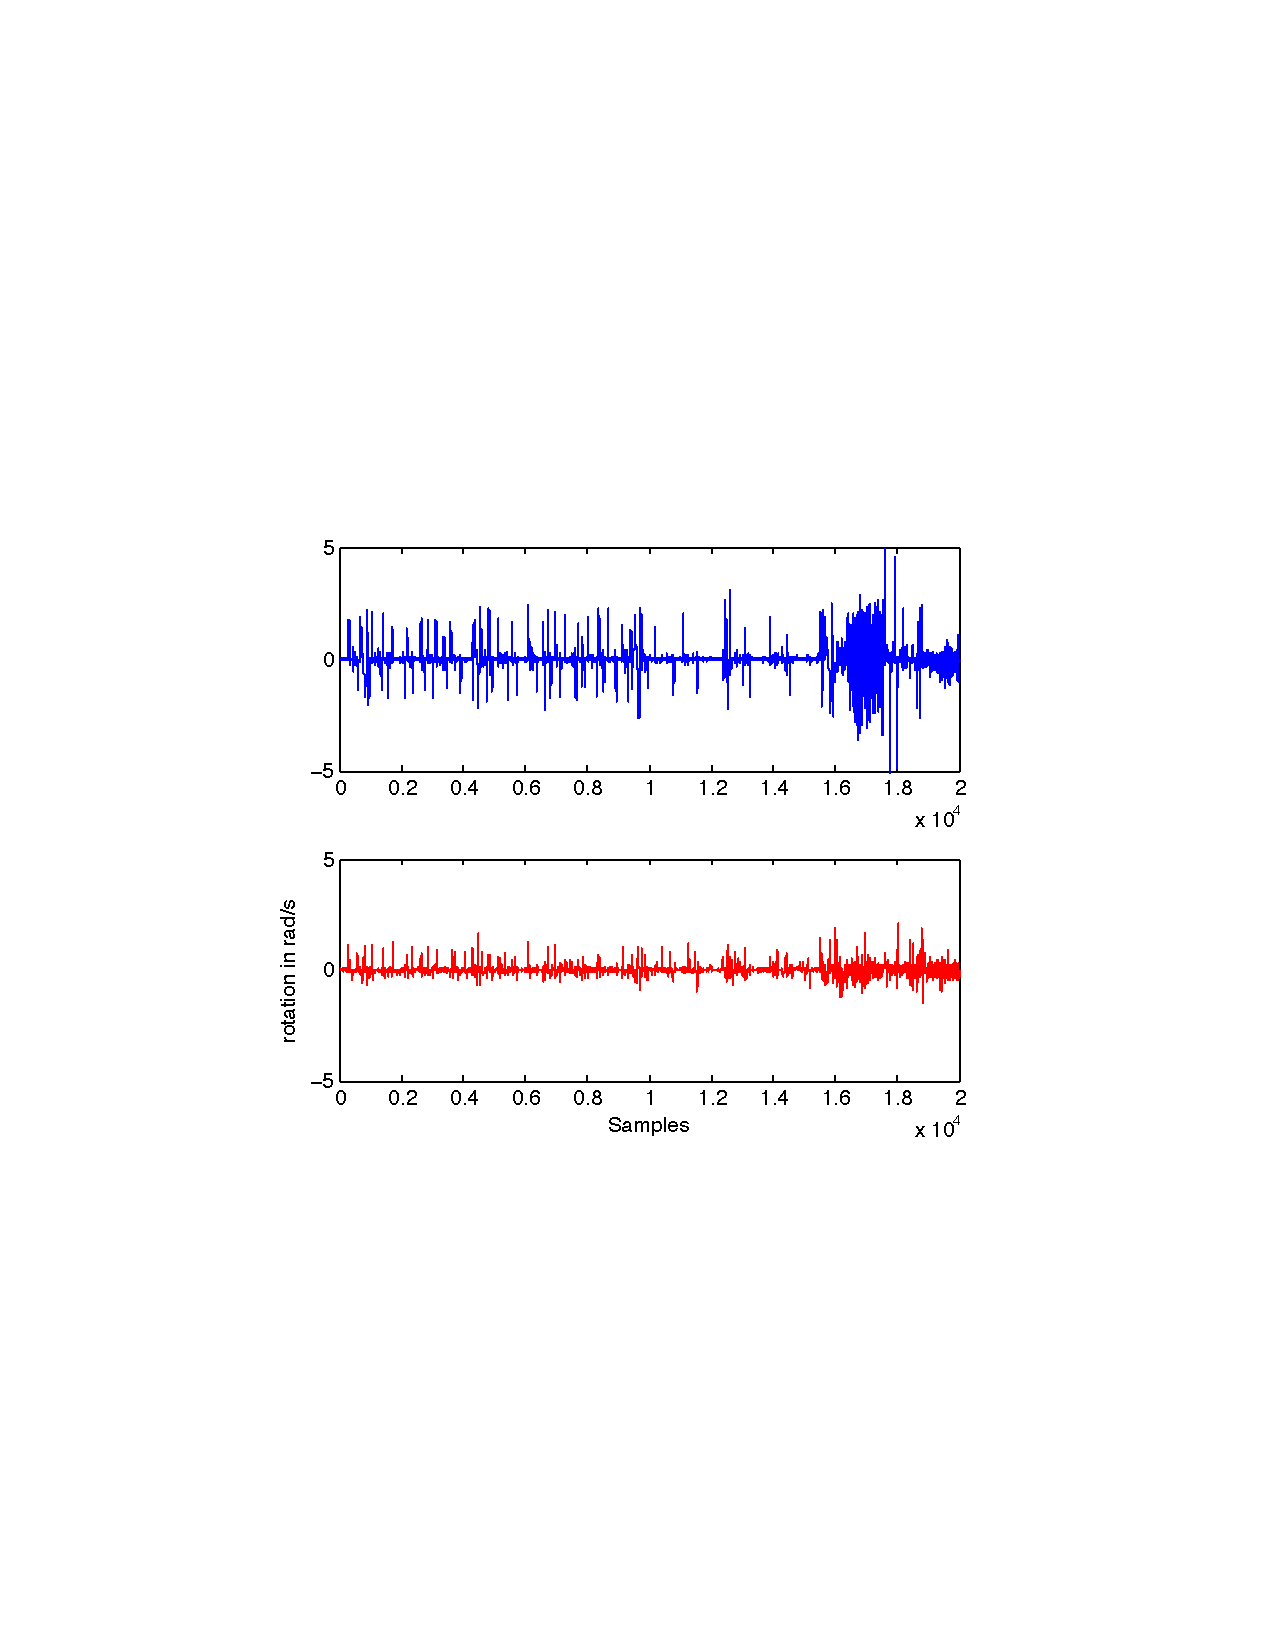
\includegraphics[width=0.95\linewidth]{drinking}
\caption{Gyro Signal, horizontal axis for drinking gestures, on the top a sensor attached to the lower arm, on the bottom a sensor attached to the left side of the head. Although the movement is closely related, as drinking involves also tilting the head, the signals are clearly distinguishable. Sampling frequency 30 Hz.}
\label{drinking}
\end{figure*}


\begin{figure*}[!t]
\centering
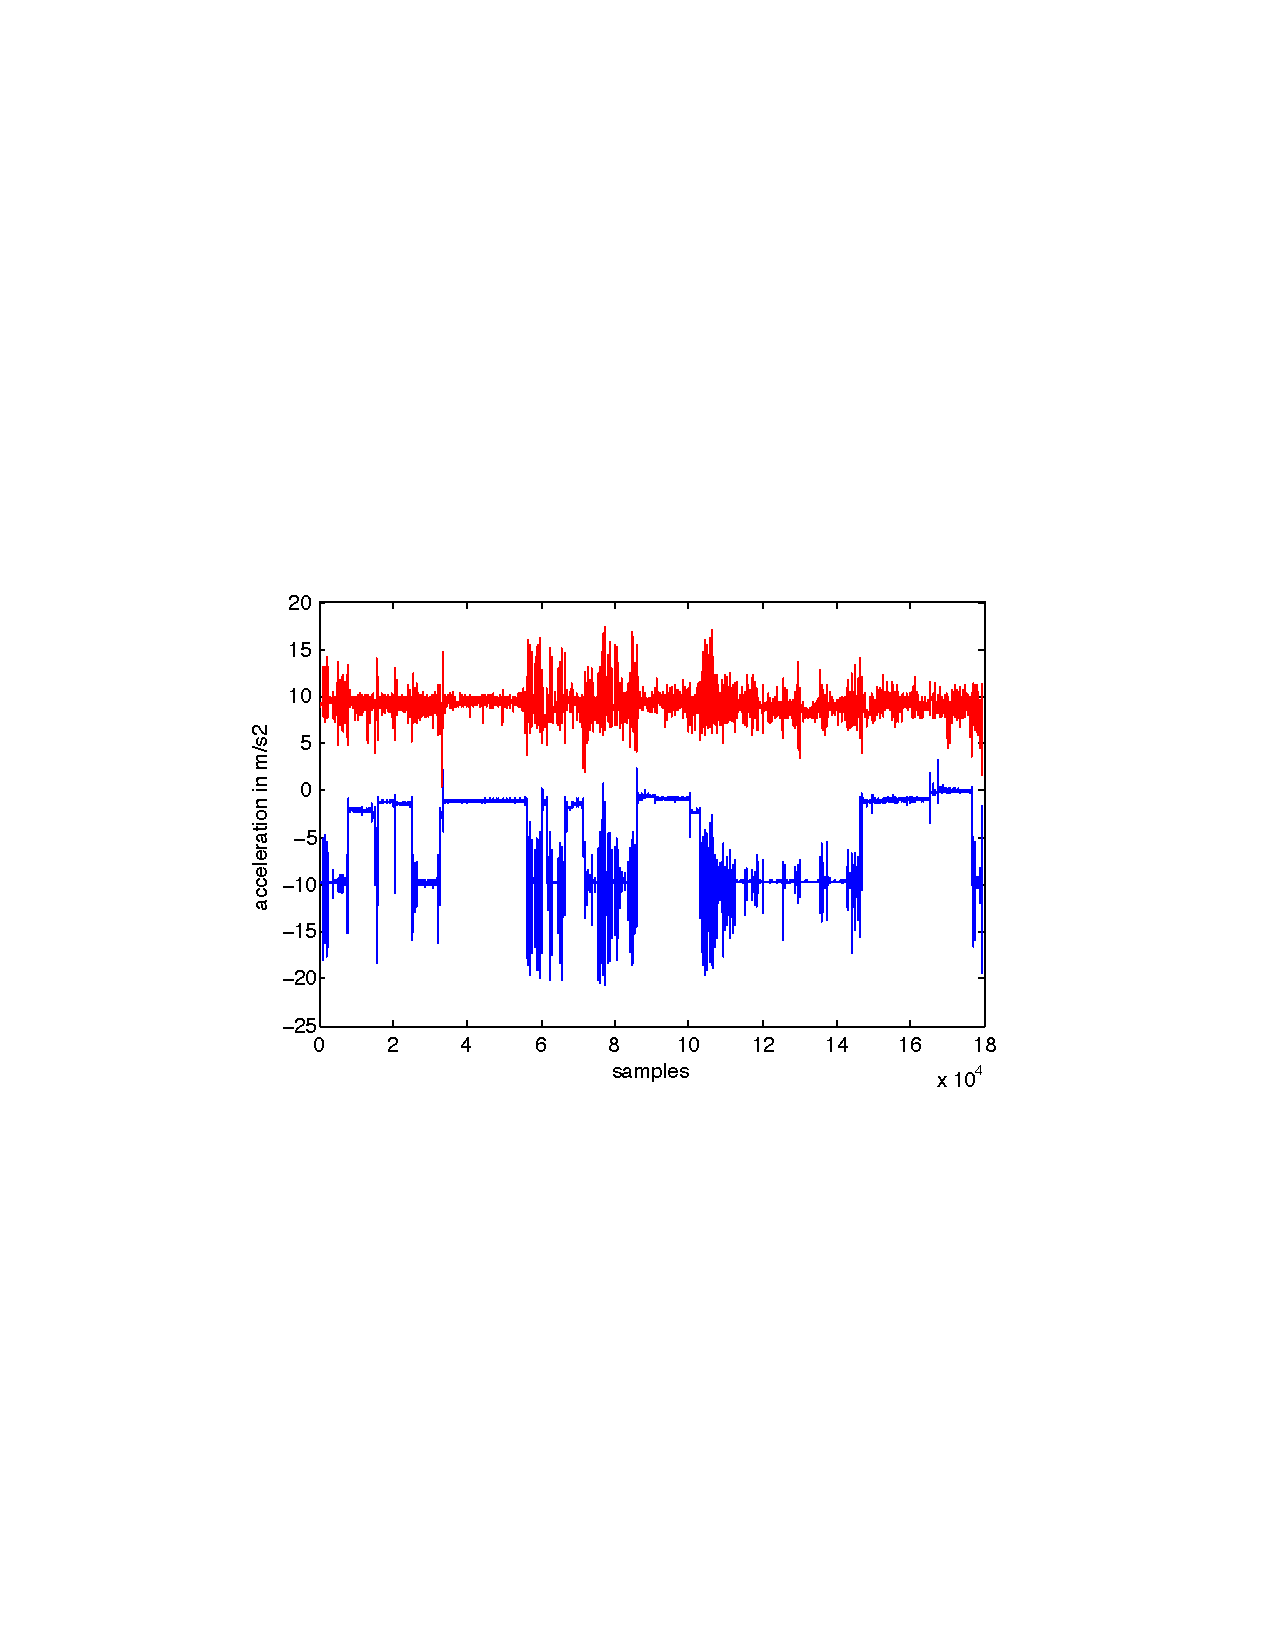
\includegraphics[width=0.95\linewidth]{acceleration}
\caption{Accelerometer signal, horizontal axis, on the top a sensor attached to the wrist, on the bottom a sensor placed in the right
trouser pocket. One can clearly see the sitting sections and the shifts in the gravity vector due to orientation changes of the sensor.
Sampling frequency 50 Hz.}
\label{acceleration}
\end{figure*}

\section{Dampening Effects}


\subsection{Sound Waves}


\begin{figure*}[hbt]
\centering
\includegraphics[width=0.95\linewidth]{frequencies}

\caption{Frequencies}
\label{FigFrequencies}
\end{figure*}

\begin{figure*}[hbt]
\centering
\includegraphics[width=0.95\linewidth]{audioPlace}

\caption{ Locations (A: Belt, B: Sports Jacket, C: Golf Trousers, D:
  Leather Jacket, E: Jeans, F: Ideal Recording)}
\label{FigLocations}
\end{figure*}


\begin{figure}[hbt]	% remove '*' for one-column image
\centering
\includegraphics[width=\linewidth]{audio}
\vspace{-10pt}
\caption{Classification rates when training data and test data
are not from the same location (\textit{training data / test data)}}
\vspace{-10pt}
\label{FigMixedTrainingTesting}
\end{figure}	

We investigate how different locations inside clothing influence the ability of a system to recognize activity relevant sounds. Specifically, we consider the recognition of sounds from 9 household and office appliances recorded using an iPhone placed in 2 trouser pockets, 2 jacket pockets, a belt holster and the users� hand. The aim is not to demonstrate good recognition rates on the above sounds (which has been done many times before) but to compare recognition rates from the individual locations and to understand how to best train the system to be location invariant.

When trained and tested on the same location the results were between
90\% (leather jacket) and 97\% (golfing trousers and hand) for frame by frame recognition and between 98\%
(interestingly for the clean data) and 100\% (for all the
others) for the majority decision. This clearly shows that the answer to our first question is yes: it
is feasible to do good quality recognition with the phone inside
clothing.

Figure~\ref{FigMixedTrainingTesting} shows the results of testing on
different locations when the system was trained on the 'clean' (in the
hand) data and on a mix of data from all locations (except the one on
which it was tested).  The results for 'clean'
training are poor for both frame by frame and majority decision (around 60\%). 
 This
shows that the damping induced through clothing has a significant
influence on the spectral composition of the sound  and  has to be
appropriately modeled to achieve reasonable performance.   The effect
of the damping depends on the sound. While microwave, printer, toilet
flush, coffee grinder and background had a recognition rate of 90\% to
100\%, the rates for the remaining sounds dropped to 0 (hot air gun) 10\%
(water tap and water boiler) and 5\% (drill).



\subsection{RadioFrequencies}

\begin{figure*}[hbt]
\centering
\includegraphics[width=0.95\linewidth]{wavelength2}
\caption{Wavelengths for part of the frequency spectrum}
\label{FigRadio}
\end{figure*}


Very High Frequency Range (WLAN) and Ultrahigh Frequency Range (GPS).

\subsubsection{Wireless LAN}

\subsubsection{Global Positioning System}


We present an elaborate experimental study of the influence of device
placement on the GPS location accuracy in three different mobile
appliances: iphone 3gs, nokia n95 and nokia 810. 
On a total of some 52 km of walking traces  we shaw that there are
statistically significant difference in the errors between 5 on body
locations: hand, front pocket of trousers, inner pocket of the jacket, inside a
backpack. While the fact that such difference exists was well known
before,  this paper is the first to systematically study the effect.


GPS receivers are increasing becoming a standard feature in mobile smart
phones. This enables a broad range of new applications ranging from
a personal assistant reminding the user to buy groceries on his way
home through pervasive advertisement~\cite{Schiller:2004p8797} to
sports performance monitoring (how far and how fast did I run?).
What such applications have in common is that the usage mode of the
GPS system is different from a standard way finding task. In the
latter the device is mostly being used when hand held. In the former,
it is expected to  reliably follow the user's location while
carried in a pocket, bag or holster.  This raises the question of
signal quality. Obviously, human body contributes to signal
attenuation and the fact that GPS  location accuracy will be different
depending on where the device is placed is well known. 
However, while there has been 
several studies of GPS accuracy, (\cite{Kihara:1994p8400,Matsushita:2009p8335}) 
the effects of device placement has so far
not been systematically studied. Thus, while it is known that some sort
of effect is to be expected, the extent is unclear.  In this paper, we
present a systematic experimental evaluation of the effect.

\begin{figure}[t]
    \begin{center}
    \subfloat[]{\includegraphics[width=0.40\linewidth]{normalx.png}
    	\label{fig:normalx}}
     \subfloat[]{\includegraphics[width=0.40\linewidth]{normaly.png}
    	\label{fig:normaly}}
      \end{center}
\caption[]{
Error distribution for several traces with x being the error in meters and y the sample number.
\ref{fig:normalx} shows the error distribution for the iphone 3gs, \ref{fig:normaly}  for the nokia 810.}
\label{fig:normal}
\end{figure}

\begin{figure}[!t]
\centering
\begin{center}
    \subfloat[]{\includegraphics[width=0.40\linewidth]{city1_overview.pdf}
    	\label{fig:city1}}
     \subfloat[]{\includegraphics[width=0.4\linewidth]{field2.png}
    	\label{fig:field2}} \\   \end{center} 
     \subfloat[]{\includegraphics[width=0.4\linewidth]{city2_overview.png}
    	\label{fig:city2}}
     \subfloat[]{\includegraphics[width=0.4\linewidth]{woods.png}
    	\label{fig:woods}}
     \caption{Sample tracks used for the experiments. The two city tracks are depicted in~\ref{fig:city1} and~\ref{fig:city2}, one of the field tracks
     in~\ref{fig:field2} and the wood track in~\ref{fig:woods}. }
\label{fig:citytrace}
\end{figure}

\begin{figure}[!t]
\centering
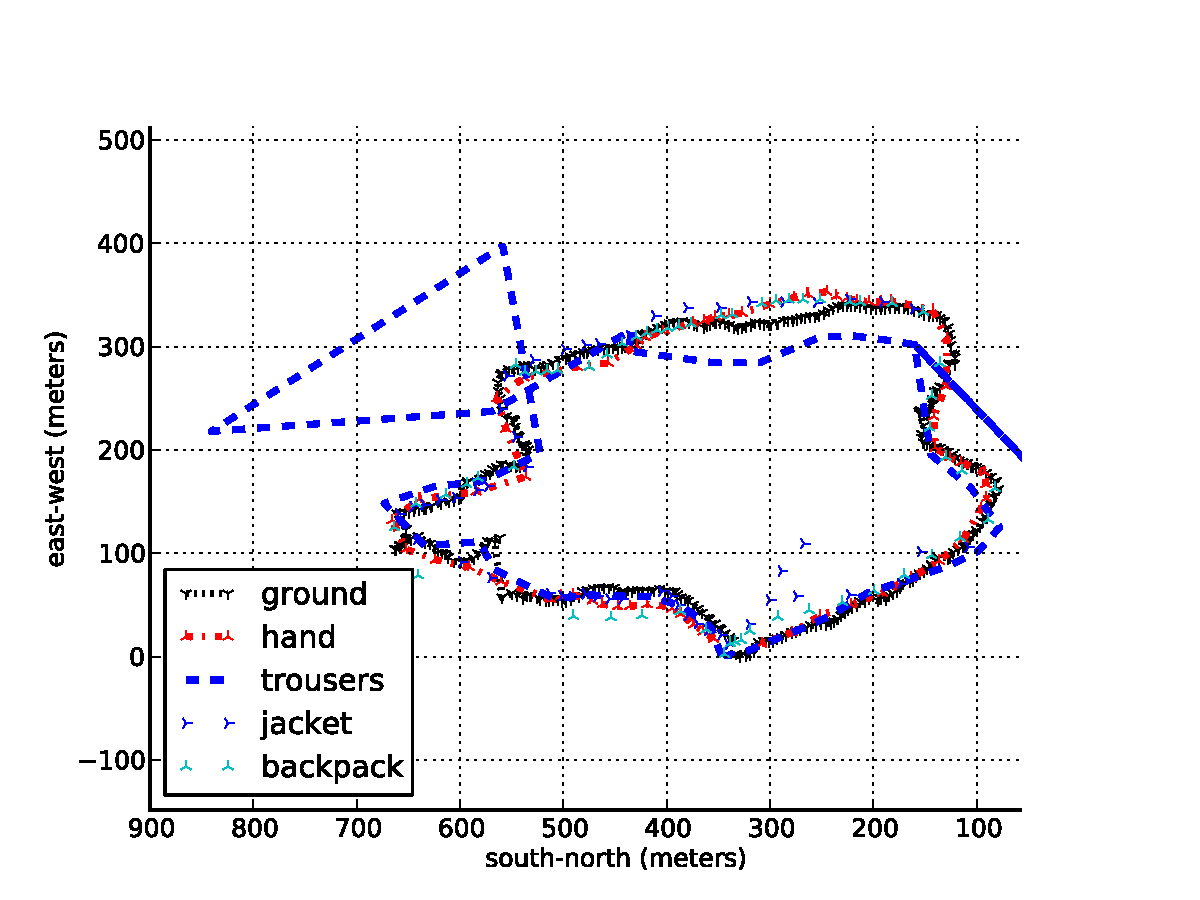
\includegraphics[width=0.95\linewidth]{city2}
\caption{Representative data trace from the iphone 3gs}
\label{fig:city}
\end{figure}

For the experiments, we pick 3 commodity GPS appliances, the iphone 3gs, the nokia n95 and
the nokia 810i. For "ground truth" as a comparison we use the Garmin Forerunner 405, 
placed on the wrist, as it provides higher accuracy GPS according the the specifications. 
The test devices are placed in each of the following locations:
hand, front pocket of trousers, inner pocket of the jacket, inside a
backpack.
The locations are picked according to a study by Ichikawa et. al.
\cite{Ichikawa:2005p6295}. They have investigated the most common places
users carry their mobile phones. 
We recorded total of five different tracks each around 2-3 km. We picked two 
tracks in cities where high buildings and narrow streets are interfering with the signal, 
two tracks in the open field, and a forest track with blocking trees. We believe these tracks are 
quite representative  for a large variety of use cases.

We record each track four times with each device in each location, in total over 52 km. 
The error of each device at each location is computed in meter by
comparing the output with the hand held Garmin Forerunner device.

Although the raw GSP error is not normal distributed(see~\cite{Michalski:2004p8514}),
we can assume a normal distribution for the relative error between the mobiles and
our reference GPS device. Depicting the different error distributions (see Figure~\ref{fig:normal}),
they can be estimated well using a Gaussian.
Therefore,  A standard  t-test can be used for any  two samples to check if 
the differences in performance is statistically significant. 




The iPhone 3GS was the most accurate of the tested mobiles. This is mostly due
to the fact that it uses assisted GPS.
The Nokia 95 was the worst in these tests. Interestingly, for this
device  the performance  was  not in  the hand, but the jacket. 
In the overall statistics, as expected the hand is the best place, jacket and backpack 
are almost equivalent, with the backpack being a little worse. The trousers is the worst.
The details for each device are given in Table~\ref{all_prob} and Figure~\ref{fig:mean}. 

\begin{table}[ht]
  \centering
\begin{tabular}{|c||c|c|c|}
\hline
On-Body Location & Mean error & Variance & Number of Points \\
\hline
\hline
Hand & 5.67m & 15.22 & 626 \\
Trousers & 8.16m & 33.97 & 483 \\
Jacket & 7.27m & 47.36 & 527 \\
Backpack & 6.34m & 36.51 & 540 \\
\hline
\hline
\hline
On-Body Location & Mean error & Variance & Number of Points \\
\hline
\hline
Hand & 6.72m & 37.93 & 3302 \\
Trousers & 9.61m & 32.29 & 2209 \\
Jacket & 5.78m & 21.58 & 2690 \\
Backpack & 6.83m & 26.39 & 3172 \\
\hline
\hline
\hline
On-Body Location & Mean error & Variance & Points \\
\hline
\hline
Hand & 6.85m & 31.28 & 4759 \\
Trousers & 8.68m & 57.21 & 5171 \\
Jacket & 8.57m & 56.98 & 5173 \\
Backpack & 9.67m & 64.10 & 5029\\
\hline
\hline
\end{tabular}	
  \caption{Data Summary for the iPhone 3GS, Nokia 810i and N95 (from top to bottom). 
  The tables include the mean error, the variance and number of GPS points logged.}
  \label{all_prob}
\end{table}


\begin{table}[ht]
  \centering
    \begin{tabular}{|c||cccc|}
\hline
 On-Body Location& Mean error & Variance &Std & Points \\
\hline
\hline
Hand & 6.41m & 32.38 &5.69 & 8687 \\
Trousers & 8.82m & 48.79 &6.98 & 7863 \\
Jacket & 7.21m & 47.22 & 6.87 & 8390 \\
Backpack & 7.61m & 52.24 &7.23 & 8741 \\
\hline
\end{tabular}
  \caption{Data Summary over all mobiles and all tracks including the mean error difference,
  the variance, standard deviation and number of GPS points logged.}
  \label{overall_data}
\end{table}


\begin{table}[ht]
  \centering
\begin{tabular}{|c||c|c|c|c|}
\hline
& Hand & Trousers & Jacket & Backpack\\
\hline
\hline
Hand & & 100\% & 86.9\% & 95.4\% \\
\hline
Trousers & 100\% & & 98.8\% & 95.4\% \\
\hline
Jacket & 86.9\% & 98.8\% & & 71.2\% \\
\hline
Backpack & 95.4\% & 95.4\% & 71.2\% & \\
\hline
\end{tabular}	
  \caption{Stochastic independence of the expectancy values gotten from all tracks and all mobiles}
  \label{overall_prob}
\end{table}


\begin{figure}[!t]
\centering
\includegraphics[width=0.75\linewidth]{mean}
\caption{Mean distance error and standard deviation over all mobiles.}
\label{fig:mean}
\end{figure}

Performing a T-test over all data shows that the error on  most of the
on-body locations can be seen as coming from a different probability
distribution. In other words, the performance difference can be seen
as statistically significant.


We show that the differences in the GPS positioning error  dependent on the on-body device placement 
are statistically significant.
A very interesting finding is that the placement with the highest variance 
and worst reception in our experiments is in the trousers. The front trousers pocket is according
to Ichikawa et.al.~\cite{Ichikawa:2005p6295} the most likely placement users carry their mobile.
This is important to keep in mind. Researchers and developers should use the on-body location they expect the 
users to put their GPS receiver for any experimental setup or application development tests.

Future work includes detecting the on-body placement (see~\cite{Kunze:2007p86} for details on how this can be achieved) 
and modeling the error depending on the position to compensate for it, if necessary.

This paper is part of a larger effort from our lab to point out and deal with
the variances and differences in signals from body sensor networks 
depending on the on-body placement.
 

\section{In Summary}



